% INNAN DU COMMITAR!
% Uppdatera datum
% Uppdatera version
%-----
% Document name



\documentclass[10pt,a4paper]{article}
\usepackage[utf8]{inputenc}
\usepackage[english]{babel}
\usepackage{amsmath}
\usepackage{amsfonts}
\usepackage{amssymb}
\usepackage{graphicx}
\usepackage{geometry}

\title{PostCardBuddy}
\author{Team C}

\begin{document}
\begin{titlepage}
\newgeometry{left=2cm,top=1cm,right=2cm}
\newcommand{\HRule}{\rule{\linewidth}{0.5mm}}


\begin{flushright}
November 20, 2015 v0.06\\[3cm]
\end{flushright}


\centering
\textsc{\LARGE Team C}\\[0.5cm]

\HRule \\[0.4cm]
{ \huge \bfseries PostCardBuddy}\\[0.3cm]
{\Large \bfseries System Requirements}\\[0.4cm] % Title of your document
\HRule \\[1.5cm]

\vfill
\begin{flushleft}
%Authors, write on separate lines
\textit{Authors of this document:}\\
Emma Albertz\\
Caroline Brandberg\\
Linnéa Claesson\\
Billy Johansson\\
Johan Ju\\
Jacob Mejvik\\
Carl Rynegardh
\end{flushleft}

\end{titlepage}
\pagenumbering{gobble}



%\begin{center}
%\textit{\large Version History}
%
%    \begin{tabular}{ | l | l | l | p{5cm} |}
%    \hline
%    \textbf{Version} & \textbf{Date} & \textbf{Responsible} & \textbf{Description} \\ \hline
%    1.0 & 2015-10-14 & EA, LC & Baseline\\ \hline
%    \end{tabular}
%\end{center}



\setcounter{tocdepth}{2}
\tableofcontents
\newpage
\pagenumbering{arabic}


%--------------------------------------------------------------------%
%----------------- System Requirements ------------------------------%
%--------------------------------------------------------------------%
% Different types of system requirements (e.g. data, function, quality) at different levels (e.g. goal, domain, product, design).
% Each requirement should have a unique identity (name or number) that is consistent between releases.
% A subset of the requirements should be prioritized.

% 3A) more than two types of requirement (e.g. data, function, quality), and more than three abstraction levels (e.g. goal, domain, product, design) 
% 4A) combine different degrees of completeness and different levels of abstraction
% 4C) provide explicit requirements rationale that reduce risks of misinterpretation.
% 4D) use hierarchies and requirements relations to manage evolving requirements structures.
% 5G) use prioritization to focus improvements of specification quality and elicitation efforts for a well motivated subset of requirements.
\section{System Requirements}

\subsection{Goal}
The product aims to increase the amount of postcards sent and will achieve this through the following goals:
\begin{itemize}
\item Simplify the process of sending postcards
\item Enable user to send personalized postcards
\item It shall be possible to generate revenue through the system
\end{itemize}

\subsection{Domain}
\subsubsection{Supported systems}
\begin {description}
\item [Req 1.2.1.1] The system shall support iOS.
\item [Req 1.2.1.2] The system shall support Android.
\item [Req 1.2.1.3] The system shall support a mobile payment solution. 
\end{description}
\subsubsection{Interfaces}
\begin {description}
\item [Req 1.2.2.1] The interface connecting PostcardBuddy and the printed postcards is an of the shelf printer.
\item [Req 1.2.2.2] The system sends image files to a printer. 
\item [Req 1.2.2.3] 
\end{description}
\subsection{Product}
\begin{description}
\item [Req 1.3.1.1 Success notification]The user should be notified when an order is sent from a device.
\item [Req 1.3.1.2 Fail notification] The user should be notified when an order fails to be sent from a device.

\item [Req 1.3.1.3 No internet] If the user places an order on a device that is not connected to the internet, the order should be stored and sent the next time the device receives internet connection. 

\end{description}


\subsection{Design}
% Är dethär tillräckligt specifikt? Vill man ha en exempel bild och ett krav som säger att vykortet ska följa formtet?
\begin {description}
\item[Req 1.4.1.1 Front page] The front of the postcard should be a single field containing an image.
\item [Req 1.4.1.2 Text field] The back of the postcard should contain a text field.
\item [Req 1.4.1.3 Address field] The back of the postcard should contain an address field.
\item [Req 1.4.1.4 Postage field] The back of the postcard should contain a postage field. 
\item [Req 1.4.1.5 Postage print] The postage should be printed in the top right corner on the back of the postcard. 
\end{description}
\subsection{Data Requirements}
% Indata: Utseende på frankering (tänk "porto betalt" bild), bilddatabas till framsidan. 
\subsection{Function Requirements}
\subsection{Quality Requirements}
\newcommand{\tsss}{\thesubsubsection}
\subsubsection{Quality grid}
\begin{table}[]
\centering
\caption{Quality grid}
\label{my-label}
\begin{tabular}{|l|l|l|l|l|l|}
\hline
\textbf{\begin{tabular}[c]{@{}l@{}}Quality factors -\\ PostCardBuddy\end{tabular}} & \textbf{Critical} & \textbf{Important} & \textbf{As usual} & \textbf{Unimportant} & \textbf{Ignore} \\ \hline
\textbf{Operation}                                                                 &                   &                    &                   &                      &                 \\ \hline
Integrity/Security                                                                 &                   &                    & 1                 &                      &                 \\ \hline
Reliability/availability                                                           &                   & 2                  &                   &                      &                 \\ \hline
Usability                                                                          & 3                 &                    &                   &                      &                 \\ \hline
Internet connection demand                                                         & 4                 &                    &                   &                      &                 \\ \hline
Efficiency                                                                         &                   &                    & x                 &                      &                 \\ \hline
\textbf{Miscellaneous}                                                             &                   &                    &                   &                      &                 \\ \hline
Installability                                                                     &                   & 5                  &                   &                      &                 \\ \hline
Interoperability                                                                   &                   & 6                  &                   &                      &                 \\ \hline
\end{tabular}
\end{table}
\subsubsection{Performance}
\begin{description}
	\item[Req \tsss.1 Memory usage] The application shall adjust its memory usage depending on the device.
	\item[Req \tsss.2 Speed] The user interface shall be considered smooth on devices faster than Nexus 5 / iPhone 5 for 8 out of 10 users. 
	\item[Req \tsss.3 Picture quality] The camera shall be able to take a picture in the highest hardware supported resolution. 
	\item[Req \tsss.4 Autofocus] The camera shall have a autofocus that is comparable to the Android / iOS stock camera. 
\end{description}
\subsubsection{Availability}
\subsubsection{Security}
\begin{description}
	\item[Req \tsss.1 Store cards] The photos shall be stored encrypted
	%om vi kör med backend server
	\item[Req \tsss.2 Sending card] The photos shall be sent encrypted to back-end.
\end{description}
\subsubsection{Maintainability/Portability}
\begin{description}
	\item[Req \tsss.1 Language] The application shall be developed in non native language e.g. Java for Android. 
	\item[Req \tsss.2 Device support] The application shall work on devices with newer operating systems than Android 4.1 / iOS 7.0.1
\end{description}
\subsubsection{Usability}
\begin{description}
	\item [Req \tsss.1 User friendly] 9 out of 10 users shall be able to use the system after a five minute instruction.
\end{description}


\subsubsection{Usability}
\begin{description}
\item [Req 1.7.5.1 User friendly] 9 out of 10 users should be able to use the system after a five minute instruction.
\end{description}





%--------------------------------------------------------------------%
%--------------- Specification Techniques ---------------------------%
%--------------------------------------------------------------------%
% Several different specification techniques (e.g. context diagrams, features, virtual windows, task descriptions).

% 3A) apply more than one suitable specification technique (e.g. task descriptions and screen prototypes)
% 4B) use at least four different specification techniques adequately tailored to the context.
% 3B) define a system’s boundaries and its interaction with external entities.
% 5A) combine specification techniques in an explicitly motivated trade off between qualities and costs, where a high degree of specification completeness is achieved for a carefully selected subset of requirements.
% 5C) go beyond initial stakeholders and given frames, while challenging the domain boundaries and eliciting creative ideas and deep domain knowledge in real-world contexts.
\section{Specification Techniques}
\subsection{Context Diagrams}
Figure~\ref{fig:context} shows the context diagram. This diagram shows the interface that the application PostCardBuddy will interact with and the stakeholders who will interact with the application.

\begin{figure}[h!]
\centering
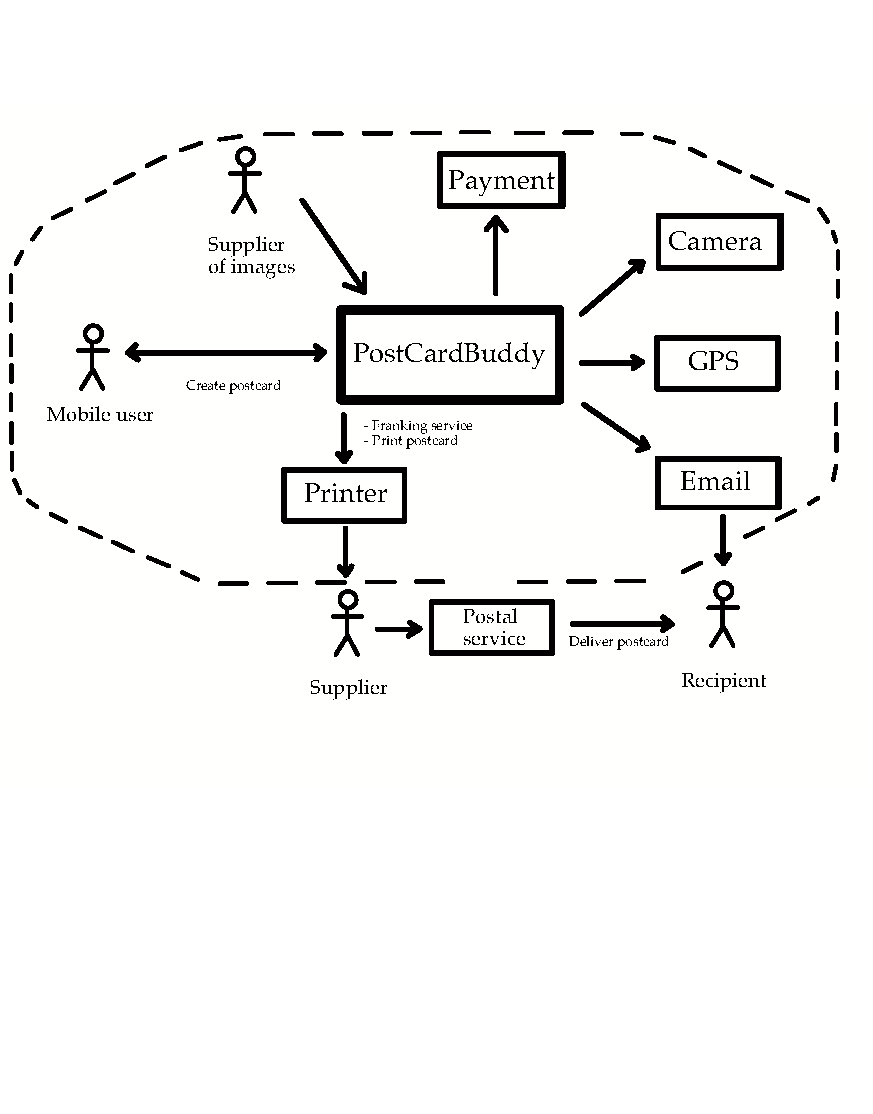
\includegraphics[width=0.7\textwidth]{ContextDiagram2.pdf}
\caption{Context diagram}
\label{fig:context}
\end{figure}

\subsection{Features}
\subsection{Virtual Windows}
\subsection{Task Descriptions}


%--------------------------------------------------------------------%
%------------------ Release Plan ------------------------------------%
%--------------------------------------------------------------------%
% A release plan defining which requirements that are implemented in each of three releases, namely R3 (final release for this course project), and the imagined future releases R4 and R5. The release plan shall include information used to derive the plan such as priorities and cost.
% The requirements planned for R3 (in the release plan) should be implemented as mock-up designs (e.g. screens and prototypes, analog drawings, clickable presentations, executable gui mockups) and thus included in the final (R3) release.

% 4H) create a release plan for a subset of prioritized features, while taking into account precedence constraints.
% 5F) combine priorities from several stakeholders and use priorities and scheduling constraints to iteratively create a relevant release plan.
\section{Release Plan}




\end{document}

